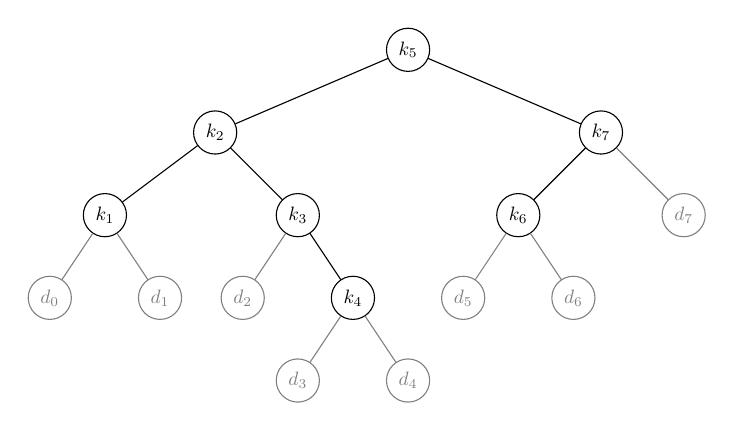
\begin{tikzpicture}[scale=0.7,every node/.style={scale=0.7}]
\tikzstyle{tnode}=[circle,draw,minimum width=0.5cm];
\tikzstyle{dnode}=[tnode,gray];

\node [tnode] (v1) at (2,1.5) {$k_5$};
\node [tnode] (v2) at (-1.5,0) {$k_2$};
\node [tnode] (v3) at (-3.5,-1.5) {$k_1$};
\node  [dnode] (v4) at (-4.5,-3) {$d_0$};
\node [dnode] (v5) at (-2.5,-3) {$d_1$};
\node [tnode] (v6) at (0,-1.5) {$k_3$};
\node [dnode] (v7) at (-1,-3) {$d_2$};
\node [tnode] (v8) at (1,-3) {$k_4$};
\node [dnode] (v9) at (0,-4.5) {$d_3$};
\node [dnode] (v10) at (2,-4.5) {$d_4$};
\node  [tnode] (v11) at (5.5,0) {$k_7$};
\node [tnode] (v12) at (4,-1.5) {$k_6$};
\node [dnode] (v14) at (3,-3) {$d_5$};
\node  [dnode] (v15) at (5,-3) {$d_6$};
\node  [dnode] (v13) at (7,-1.5) {$d_7$};

\draw  (v1) edge (v2);
\draw  (v2) edge (v3);
\draw [gray] (v3) edge (v4);
\draw [gray]  (v3) edge (v5);
\draw  (v2) edge (v6);
\draw [gray] (v6) edge (v7);
\draw  (v6) edge (v8);
\draw [gray] (v8) edge (v9);
\draw [gray] (v8) edge (v10);
\draw  (v1) edge (v11);
\draw  (v11) edge (v12);
\draw [gray] (v11) edge (v13);
\draw [gray] (v12) edge (v14);
\draw [gray] (v12) edge (v15);
\end{tikzpicture}